\documentclass[9pt,a4j,twocolumn]{ltjsarticle}
% 実験V報告書様式
\usepackage{experiments_v}

% ソースコード表示
\usepackage{listings}
% 色
\usepackage{xcolor}
% 数学関連
\usepackage{amsmath, amssymb}
\usepackage{bm}
% リスト制御
\usepackage{enumitem}
% newtxフォント
\usepackage{newtxmath, newtxtext}
% 画像
\usepackage{graphicx}
% shaded環境の背景色の定義
\definecolor{shadecolor}{gray}{0.80}
% 枠
\usepackage{ascmac}
\usepackage{tcolorbox}
% url表記
\usepackage{url}
% ハイパーリンク
\usepackage[pdfencoding=auto]{hyperref}
% mac用フォントセット
\usepackage{layouts/lualatexsets/fonts}
% Tikz関係
\usepackage{tikz}
% 証明などのスタイル
\usepackage{layouts/others/theorem}
% セクションの表示スタイル
%\usepackage{layouts/others/section}

% bibtex
\usepackage[backend=bibtex, style=numeric]{biblatex}
\addbibresource{lib.bib}

% ベクトル表記
\def\vector#1{\mathop{\mathbf{#1}}}
% 画像・図表等のrefコマンド
\def\thmref#1{Thm. \ref{#1}}
\def\lmmref#1{Lemma. \ref{#1}}
\def\figref#1{図\ref{#1}}
\def\eqref#1{(\ref{#1})式}
\def\tableref#1{表\ref{#1}}

%%% 著者情報 %%%
% 出席番号
\attendancenumber{32}
% 著者
\author{萩原 涼介}
% タイトル
\title{クラスタ数推定に用いる最適な情報量基準の探求}
% 指導教員
\adviser{藤田 一寿}
% 日付
\date{\today}

\hypersetup{%
  colorlinks=true,%
  urlcolor=black,%
  linkcolor=black,%
  citecolor=black,%
  linktocpage=true,%
  bookmarks=false,%
  pdftitle={情報工学実験V 報告書},%
  pdfsubject={クラスタ数推定に用いる最適な情報量基準の探求},%
  pdfauthor={Hagihara Ryosuke},%
  pdfkeywords={クラスタリング; 情報量規準; クラスタ数推定; 機械学習}
}

\begin{document}
\maketitle
\section{はじめに}
クラスタリングとはデータを教師なし学習により任意の数のクラスタに分ける手法である.
クラスタリングはデータ解析,データマイニング,パターン認識など様々な分野で用いられる.
多くのクラスタリング手法では,予めクラスタ数を指定しクラスタリングを行う.
しかし,データに対し最適なクラスタ数を指定しなければ,最適なクラスタリング結果を得ることはできない.
その為,クラスタ数を推定することは重要な課題となっている.

既存のクラスタ数推定手法の多くは,情報量規準に基づきクラスタ数の推定を行っている.
情報量規準とは簡単に言えば確率分布とデータの分布の当てはまり具合を表す.
その情報量基準は多くの研究者により様々なものが提案されている.
しかし,どの情報量規準がどのようなデータに対し有効かは分かっていない.
そこで本研究では,クラスタ数推定に用いる情報量規準として最適なものを数値実験を通し明らかにする.

\section{実験の手法}
% 4月から6月は機械学習および確率統計の基礎学習およびPythonの勉強を行った.
% 6月,7月にk-meansやx-meansの実装を行った.
% 
\subsection{k-means}
k-means\cite{macqueen1967some}は,多次元空間上のデータ点集合について,各データが属するクラスタを同定する
クラスタリング手法の一種である.
具体的には,以下の2つの手順を繰り返すことで具体的にクラスタリングを行う.
\begin{enumerate}
  \item 各データに割り当てられているクラスタのセントロイドを求める
  \item 各データ点とデータ点の距離を求め,各データ点を最も近いセントロイドのクラスタに割り当てる.
\end{enumerate}

\subsection{x-means}
x-means\cite{pelleg2000x}は,
データ分布が混合等方Gauss分布から生成されたと想定してクラスタリングを行う手法である.
k-meansの逐次繰り返しと,BIC(Bayesian Information Criterion; ベイズ情報量規準)による
分割停止規準を用いることで,クラスタ数を自動的に決定する.

データ$D$が与えられたとき,クラスタ$M$に含まれるデータ$x_i$を$K$個のクラスタに分割することを想定する.
$p$変量Gauss分布\eqref{eq:gaussian-distribution}を仮定する.
\begin{align}
  \label{eq:gaussian-distribution}
  \hat{P}(x_i) = \frac{R_{(i)}}{R}\frac{1}{\sqrt{2\pi}\hat{\sigma}^M}
    \exp\left(-\frac{1}{2\hat{\sigma}^2}||x_i-\mu_{(i)}||^2\right)
\end{align}
ここで$\mu_{i}$は$p$次の平均ベクトルである.
なお,等方Gauss分布からデータが生成されるとすると,分散は\eqref{eq:variance}により表される.
\begin{align}
  \label{eq:variance}
  \hat{\sigma}^2 = \frac{1}{R-K}\sum_i\left(x_i - \mu_{(i)}\right)^2
\end{align}
この時のBICを\eqref{eq:bic}により計算する.
\begin{align}
  \label{eq:bic}
  {\mathrm BIC}(M_j) = \hat{l}_j(D) - \frac{p_j}{2}\ln R
\end{align}

$p_j/2$はパラメータ空間の次元数であり,$R$はデータ数,
$\hat{l}_j(D)$は$p$変量Gauss分布の対数尤度関数である.

x-meansにおけるクラスタリングは以下のように行われる.
\begin{enumerate}
  \item クラスタ数を小さな値(2や3)にしてk-meansを実行
  \item 各クラスタにおけるBICを算出する
  \item それぞれのクラスタのセントロイドを2つに分割し,k-meansを再度実行
  \item 分割したそれぞれのクラスタにおけるBICを算出
  \item 分割前と後のBICを比較し,BICが大きくなっていれば採用する
  \item 2から5を繰り返し,変化がなくなればクラスタリングが完了する
\end{enumerate}

\subsection{実験手法}
実験にはPython3.5を用い,
TensorFlow1.2.1と呼ばれるオープンソースのライブラリを用いてアルゴリズムを実装した.

\section{結果}
\subsection{k-meansによるクラスタリング}
\figref{img:kmeans-before}のデータをクラスタ数3としてクラスタリングした結果,
\figref{img:kmeans-after}のような結果になった.

なお,クラスタリングの打ち切り条件は,セントロイドの差が$1.0\times10^{-10}$以下のときとした.
\begin{figure}[htbp]
	\begin{center}
		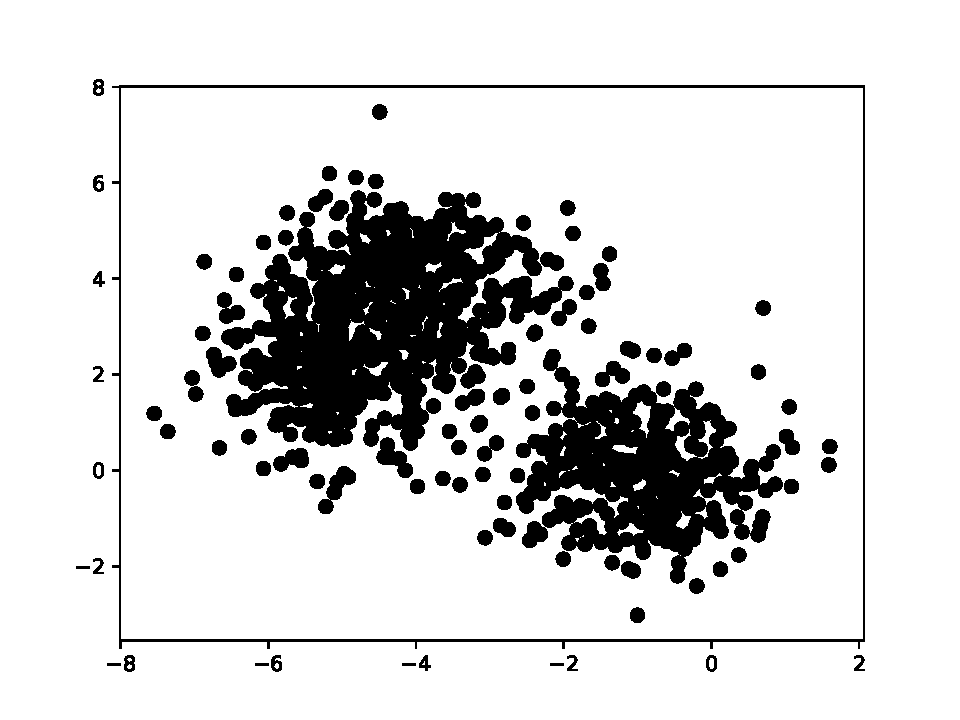
\includegraphics[width=0.8\linewidth]{img/k-means/before.pdf}
		\caption{クラスタリング前のデータ}
		\label{img:kmeans-before}
	\end{center}
	\begin{center}
		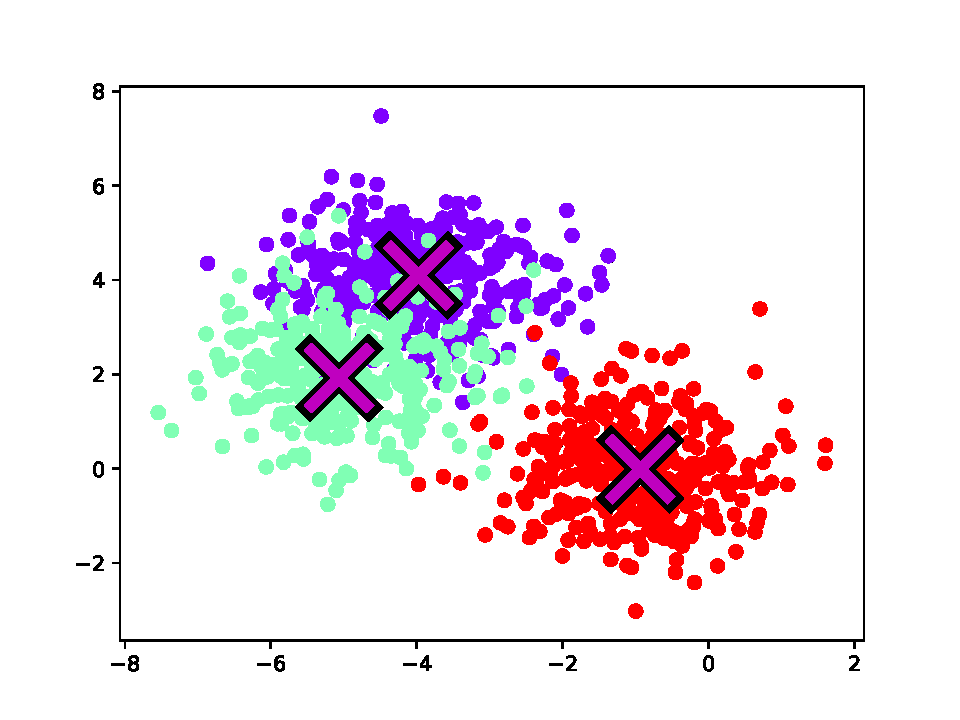
\includegraphics[width=0.8\linewidth]{img/k-means/after.pdf}
		\caption{クラスタリング後のデータ}
		\label{img:kmeans-after}
	\end{center}
\end{figure}
\section{おわりに}

\printbibliography[title=参考文献]

\end{document}
